% Recall Is the Wrong Yardstick — conference manuscript.
% Generated from PAPER_DRAFT.md; every number is traceable to results/ and is
% checked by scripts/audit_paper_numbers.py.
%
% Build:  cd AudioVQ/paper && pdflatex recall_wrong_yardstick && pdflatex recall_wrong_yardstick
\documentclass[conference]{IEEEtran}

\usepackage{booktabs}
\usepackage{graphicx}
\usepackage{amsmath,amssymb}
\usepackage{textcomp}
\usepackage{xcolor}
\usepackage{url}
\usepackage[hidelinks]{hyperref}

\graphicspath{{../results/figures/}}

\newcommand{\ie}{i.e.\ }
\newcommand{\eg}{e.g.\ }

\begin{document}

\title{Recall Is the Wrong Yardstick:\\Evaluating Data-Oblivious Vector Quantization\\on Audio Embeddings}

\author{\IEEEauthorblockN{SPARC FYP Team}
\IEEEauthorblockA{\textit{Final Year Project}\\
sparcproject2026@gmail.com}}

\maketitle

\begin{abstract}
Retrieval over audio embeddings underpins query-by-example search, acoustic-scene matching and
noise-prototype lookup, and on edge hardware the embedding index---not the model---is usually the
memory bottleneck. Data-oblivious vector quantization compresses vectors with no training pass at
all, making it attractive for indices built or extended on-device, but it is evaluated almost
exclusively by geometric recall against uncompressed nearest neighbours.
We evaluate data-oblivious quantization (random rotation followed by per-coordinate optimal scalar
quantization) on audio embeddings across three self-supervised speech models---WavLM-Base+,
wav2vec2-base and HuBERT-base---using 10\,000-vector indices from MS-SNSD and VoiceBank-DEMAND.
Our central result is a \emph{dissociation between geometry and meaning under lossy compression}.
At ${\sim}30\times$ compression the quantizer loses roughly half of the true nearest neighbours,
yet retains ${\sim}96\,\%$ of downstream speaker- and noise-type-retrieval accuracy on every model
tested. Prior work reaches the same conclusion from the \emph{search-approximation} side, showing
downstream quality is stable while Recall@$k$ falls~\cite{dimitropoulos2026}; we establish it for
the distinct and harsher case where the representation itself is destroyed, on audio, with a
measured effect size replicated across three backbones.
We also give a mechanistic account of the random rotation: it flattens a spiky \emph{within-vector}
coordinate profile (crest factor $10.2 \rightarrow 3.3$ against an isotropic ideal of $3.4$). This
produced a cross-model prediction, recorded in advance and confirmed. A third model showed the
crest factor is a reliable \emph{binary screen} for whether rotation is worth applying, but
\emph{not} a predictor of how large the gain will be---we report the weaker claim the evidence
supports. Practically, the untrained quantizer reaches $98\,\%$ of OPQ's recall at $1/434$th the
index build cost.
\end{abstract}

\begin{IEEEkeywords}
vector quantization, audio embeddings, approximate nearest neighbour search, on-device retrieval,
self-supervised speech representations
\end{IEEEkeywords}

\section{Introduction}

\textbf{Positioning.} This work sits at the intersection of two literatures that have not been
connected. The speech community has established that self-supervised audio representations are
strongly anisotropic and that their layers differ substantially~\cite{pasad2021,pasad2023,liu2024}.
The vector-quantization community has established that data-oblivious rotation-plus-scalar schemes
degrade on anisotropic embeddings~\cite{qdrant2025}. \textbf{Neither has asked what the first fact
implies for the second}, and neither evaluates audio embeddings under data-oblivious quantization.
We do not claim to have discovered either half.

\textbf{Contributions.}
\begin{enumerate}
\item \textbf{The first evaluation of data-oblivious VQ on audio embeddings}, across three
self-supervised models and two corpora. Published benchmarks of these methods cover text, image and
ads embeddings and LLM KV caches; audio is untested (Sec.~\ref{sec:related}). Existing
audio-embedding compression work uses binary hashing, LSH and PQ---all data-\emph{dependent} or
task-trained.

\item \textbf{A quantified geometry--meaning dissociation under quantization}
(Sec.~\ref{sec:dissociation}): ${\sim}50\,\%$ neighbour loss costs ${\sim}4\,\%$ of downstream task
accuracy, replicated on all three models and verified not to be an artifact of the operating point.
\textbf{This is the paper's central claim}, stated at the scope the evidence supports. We do
\emph{not} claim to be first to observe that Recall@$k$ understates deployment
quality:~\cite{dimitropoulos2026} show the same for ANN \emph{search} approximation on general
corpora and propose $1/\mathrm{Ratio}@k$ in its place. Our contribution is the harder case and the
number---search approximation returns \emph{slightly worse true vectors}, while quantization
\emph{permanently destroys representation content}, so stability under the former does not imply
stability under the latter---measured here on audio, which neither literature covers. That two
literatures reach this conclusion by different routes is corroboration, not competition.

\item \textbf{A mechanistic account of the random rotation}---the within-vector \emph{crest
factor}, a statistic the speech-anisotropy literature does not use (it reports cosine similarity
and isotropy)---validated by an advance cross-model prediction (Sec.~\ref{sec:mechanism}) and then
narrowed, over four successive tests, to a coarse per-layer threshold rather than the quantitative
predictor first claimed.

\item \textbf{An honest map of what does and does not replicate} (Sec.~\ref{sec:replication}).

\item \textbf{Three practical costs that standard reporting conceals}
(Sec.~\ref{sec:scale}--\ref{sec:layers}): the advantage of trained codebooks \emph{grows} with
index size on 3/3 models, so results at $10^4$ vectors do not transfer to $10^6$; the deployable
structured rotation loses $0.04$--$0.065$ Recall@10 at matched bits when the dimension is not a
power of two, invisible in bits-per-coordinate tables; and layer choice matters comparably for
\emph{quantized retrieval}, with the conventional final layer worst on 3/3 models.
\end{enumerate}

\section{Related work and positioning}
\label{sec:related}

\textbf{What is already known, and which we do not claim.} Three relevant facts are established.

\emph{(i)} Data-oblivious rotation-plus-scalar quantization degrades on \emph{anisotropic}
embeddings: the underlying analysis assumes vectors uniformly distributed on the sphere and does
not extend to spaces where a few directions carry most of the variance~\cite{qdrant2025}. That
source is an industry technical report rather than peer-reviewed, and we mark it as such wherever
it is load-bearing.

\emph{(i-b)} The data-oblivious regime is not a one-method field. RaBitQ~\cite{gao2024} randomly
rotates a bi-valued codebook and derives an unbiased distance estimator with a proven error bound,
and was the first practically deployable method to attain the asymptotically optimal
space--accuracy trade-off. We situate the method under test alongside it rather than presenting the
regime as unexplored. Like TurboQuant~\cite{zandieh2025}, RaBitQ is evaluated on text and image ANN
benchmarks.

\emph{(ii)} Self-supervised speech representations \emph{are} strongly anisotropic---wav2vec2
embeddings are reported as occupying a narrow cone with layerwise cosine similarities of
$0.9$--$1.0$ in upper layers~\cite{liu2024,anisotropy2026}, consistent with the $+0.83$ to $+0.93$
we measure at final layers (Sec.~\ref{sec:anisotropy}).

\emph{(iii)} Layers of these models differ substantially in what they encode, and layer-wise
analysis is an established subfield~\cite{pasad2021,pasad2023}.

We claim none of these. Our anisotropy and layer measurements reproduce known properties
\emph{in service of a question neither literature has asked}: what those properties imply for
data-oblivious quantization of audio indices.

\textbf{On evaluation metrics.} That Recall@$k$ is a pessimistic proxy is \emph{not} our
discovery.~\cite{dimitropoulos2026} show that downstream indicators---classification accuracy, RAG
answer quality---stay stable while Recall@$k$ drops substantially in ANN \emph{search}, and propose
the inverse approximation ratio $1/\mathrm{Ratio}@k$ instead. Their setting differs from ours in
the way that matters: they hold the vectors exact and vary how hard the index is searched, so a
missed neighbour is merely a \emph{slightly more distant} true vector. Under quantization the
vectors themselves are damaged and the information is gone. Stability under the first does not
entail stability under the second, and we test the second. On the compression side,
CoRECT~\cite{corect2025} benchmarks eight compression families on text retrieval up to 100\,M
passages and finds the best method varies by model---the closest existing work to
Sec.~\ref{sec:scale}, and likewise audio-free.

\textbf{What is not covered by prior work.} Published benchmarks of these quantizers use arXiv
titles, DBpedia entities, Wikipedia, product catalogues, CLIP image and ads embeddings---\textbf{no
audio}. The audio side is no better covered from its own direction: MAEB~\cite{maeb2026} evaluates
50+ audio embedding models over 30 tasks but measures \textbf{uncompressed} embedding quality only,
with no quantization, index-memory or on-device dimension. Existing audio embedding compression is
data-dependent or task-trained throughout, \eg jointly learned embeddings and balanced hash codes
for query-by-example~\cite{singh2022}.

\textbf{A distinction worth stating explicitly.} wav2vec2 and related models use product
quantization \emph{inside their own training objective} (Gumbel-softmax codebooks over encoder
features). That is unrelated to compressing utterance embeddings for a retrieval index, which is
our subject.

\section{Method}

Random rotation (Hadamard or dense Gaussian) followed by a per-coordinate Lloyd--Max quantizer
derived from the analytic post-rotation coordinate distribution; norms stored in float32 and
counted in the bit budget. Baselines: faiss PQ~\cite{jegou2011} and OPQ~\cite{ge2013} (trained on
held-out data), uniform scalar quantization, and the identical quantizer with rotation disabled as
the ablation.

\textbf{Implementation validation.} Measured MSE distortion falls below the source method's proven
upper bound~\cite{zandieh2025} at every bitrate ($b{=}1$: $0.403$ vs $0.680$; $b{=}4$: $0.0094$ vs
$0.0106$), within $2.5$--$14.4\,\%$ of its refined values. 34 unit tests cover the quantizers and
the retrieval evaluation, including brute-force verification of the top-$k$ and recall routines.

\section{Experimental setup}

Indices of 10\,000 MS-SNSD utterances with 1\,000 disjoint queries; semantic tasks use
VoiceBank-DEMAND speaker labels (824 clips) and MS-SNSD noise-type labels (1\,100 clips).
Embeddings come from pretrained WavLM-Base+~\cite{chen2022}, wav2vec2-base~\cite{baevski2020} and
HuBERT-base~\cite{hsu2021}, mean-pooled over time. Ground truth is exhaustive float32 search.
PQ/OPQ codebooks are fitted on a held-out 10\,000-vector bank, never on the vectors scored.
Comparisons use paired Wilcoxon tests and bootstrap CIs over queries.

\section{Results}

\subsection{Audio embedding spaces are extremely anisotropic}
\label{sec:anisotropy}

\begin{table}[t]
\centering
\caption{Anisotropy of the three embedding spaces at the final layer. All three occupy $1$--$3\,\%$
of their 768 ambient dimensions.}
\label{tab:anisotropy}
\begin{tabular}{lrrrr}
\toprule
 & WavLM & wav2vec2 & HuBERT & isotropic ref. \\
\midrule
mean pairwise cosine & $+0.830$ & $+0.929$ & $+0.853$ & $-0.000$ \\
effective dim. & $2.9\,\%$ & $1.4\,\%$ & $2.1\,\%$ & $92.9\,\%$ \\
\bottomrule
\end{tabular}
\end{table}

Table~\ref{tab:anisotropy} places all three models far from the uniform-on-sphere case the method
is optimal for. This confirms a known limitation (Sec.~\ref{sec:related}) in a new domain.

\subsection{Why the rotation works, and when it does not}
\label{sec:mechanism}

\begin{table}[t]
\centering
\caption{The rotation flattens a spiky within-vector coordinate profile. Rotation is worth little
on the model whose coordinates are already near-isotropic.}
\label{tab:mechanism}
\begin{tabular}{lrrrr}
\toprule
 & HuBERT & WavLM & wav2vec2 & ideal \\
\midrule
crest (raw $\rightarrow$ rot.) & $12.53{\rightarrow}3.40$ & $10.22{\rightarrow}3.34$ & $3.62{\rightarrow}3.29$ & $3.37$ \\
kurtosis (raw) & $+52.97$ & $+38.75$ & $+0.57$ & $-0.00$ \\
\midrule
\textbf{rel.\ R@10 gain} & $\mathbf{+40.2\,\%}$ & $\mathbf{+49.4\,\%}$ & $\mathbf{+2.8\,\%}$ & --- \\
\bottomrule
\end{tabular}
\end{table}

The prediction that rotation would be near-worthless on wav2vec2 was recorded \emph{before} that
benchmark ran, with the explicit condition that equal gains would falsify the mechanism
(Fig.~\ref{fig:mechanism}).

HuBERT was then added to test whether crest factor predicts the \emph{magnitude} of the gain.
\textbf{It does not}---HuBERT is the spikiest yet gains less than WavLM, inverting the predicted
ordering. We therefore report the crest factor as a \textbf{binary screen} separating ``rotation
essential'' ($\mathrm{crest} \gg 3.4$) from ``rotation near-worthless''
($\mathrm{crest} \approx 3.4$), and explicitly \emph{not} as a quantitative predictor.

\begin{figure}[t]
\centering
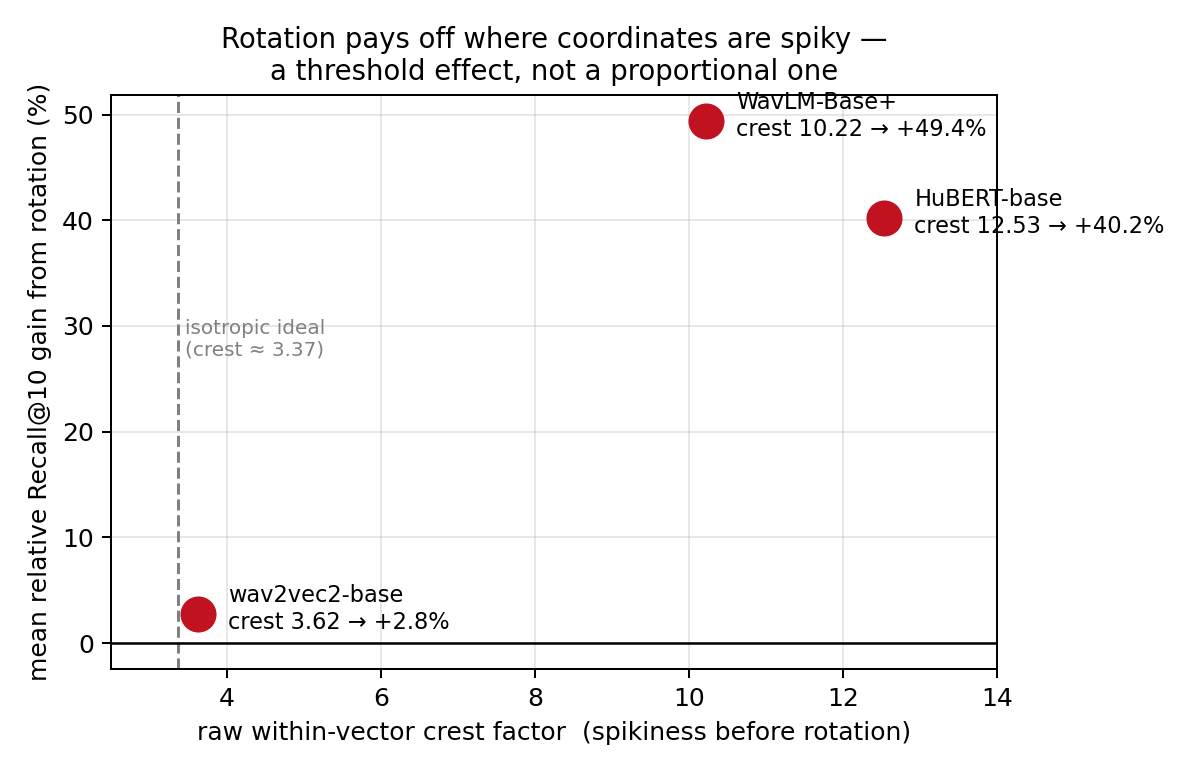
\includegraphics[width=\columnwidth]{fig8_mechanism_crossmodel.png}
\caption{Rotation benefit against raw within-vector crest factor across the three models. The
relationship is a threshold, not a proportionality.}
\label{fig:mechanism}
\end{figure}

\subsection{Geometry and meaning come apart---the central result}
\label{sec:dissociation}

\begin{table}[t]
\centering
\caption{At 1\,bit/coordinate (${\sim}30\times$ compression), roughly half the neighbour list is
destroyed while ${\sim}96\,\%$ of downstream task accuracy survives, on every model.}
\label{tab:dissociation}
\begin{tabular}{lrrr}
\toprule
model & Recall@10 kept & speaker P@10 kept & noise P@10 kept \\
\midrule
WavLM & $48\,\%$ & $96.5\,\%$ & $96.0\,\%$ \\
wav2vec2 & $53\,\%$ & $95.7\,\%$ & $96.9\,\%$ \\
HuBERT & $70\,\%$ & $\mathbf{98.6\,\%}$ & $\mathbf{97.3\,\%}$ \\
\bottomrule
\end{tabular}
\end{table}

What compression removes is largely the fine ordering \emph{among near-ties}, which the downstream
task does not depend on (Table~\ref{tab:dissociation}, Fig.~\ref{fig:central}).

\begin{figure}[t]
\centering
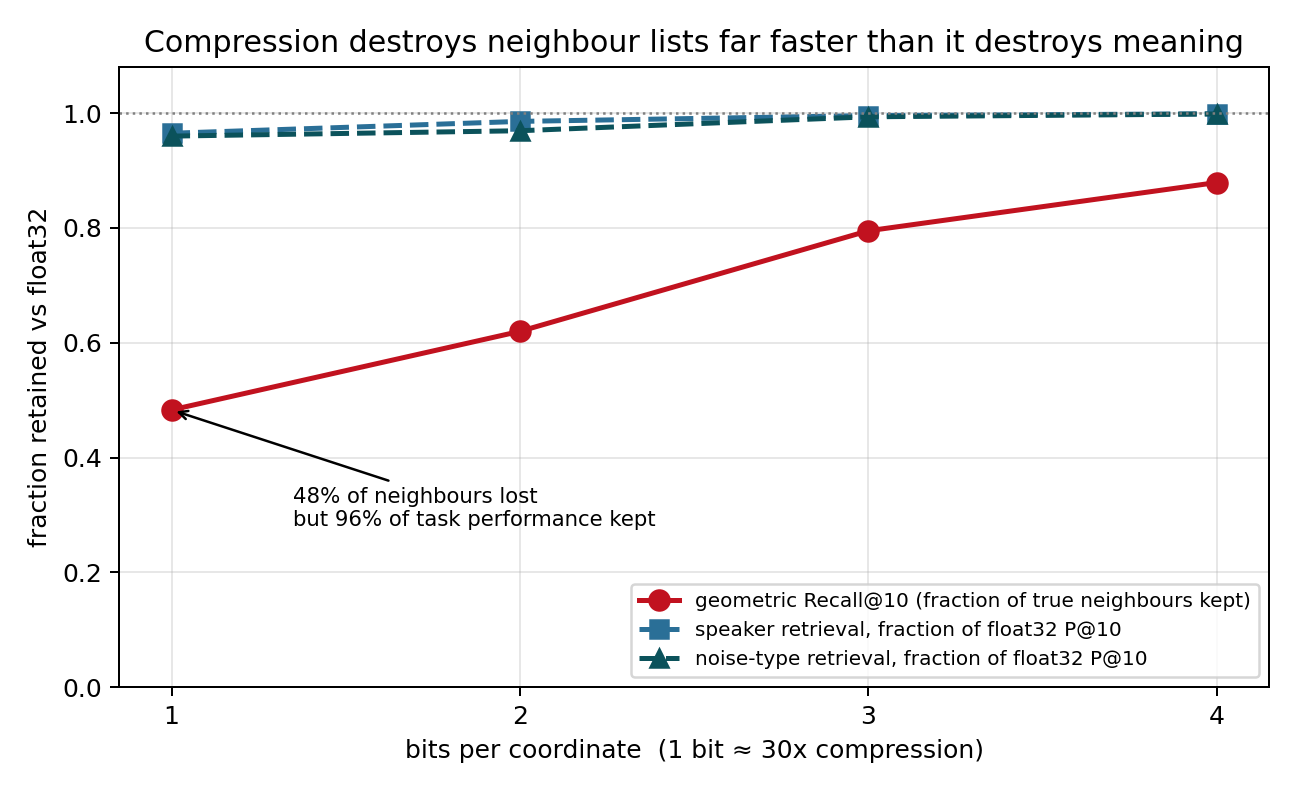
\includegraphics[width=\columnwidth]{fig5_geometry_vs_meaning.png}
\caption{Recall retention collapses with bit-width while both semantic curves stay near $1.0$.}
\label{fig:central}
\end{figure}

\textbf{Not an artifact of the operating point.} Sec.~\ref{sec:layers} shows the final layer---used
for all results above---is the \emph{worst} of twelve for retrieval, which raises the possibility
that the dissociation only appears at a poor operating point. Repeating the measurement on WavLM's
best layer (layer 2) shows the effect is if anything \textbf{stronger} there: $62.3\,\%$ of
neighbours retained against $\mathbf{99.7\,\%}$ of speaker-retrieval and $97.5\,\%$ of
noise-type-retrieval accuracy. The dissociation is a property of quantization, not of the layer
chosen.

\subsection{What replicates, and what does not}
\label{sec:replication}

\begin{table}[t]
\centering
\caption{Replication status of each finding across the three models.}
\label{tab:replication}
\begin{tabular}{p{0.52\columnwidth}p{0.38\columnwidth}}
\toprule
finding & replication \\
\midrule
geometry--meaning dissociation & \textbf{3/3 models} \\
data-dependent advantage widens as budget shrinks & \textbf{2/3 cleanly} (HuBERT non-monotone, $\rho = -0.60$) \\
rotation's task-dependent sign-flip, \emph{as scoped to spiky spaces} & \textbf{2/2 spiky models}; inert on the flat model, as predicted \\
\bottomrule
\end{tabular}
\end{table}

The sign-flip deserves comment as a methodological point. Observed first on WavLM, it failed to
replicate on wav2vec2; rather than generalise or discard it, we scoped it to spaces where the
rotation does substantial work ($\mathrm{crest} \gg 3.4$) and noted that wav2vec2 is inert by
construction. HuBERT---run afterwards, and the spikiest model of the three---reproduced the WavLM
pattern exactly: rotation significantly \emph{helps} speaker retrieval ($p \le 0.024$ at 2--4 bits)
and significantly \emph{hurts} noise-type retrieval ($p \le 3.3\mathrm{e}{-3}$ at 1--3 bits). The
scoped claim was recorded before that test and survived it; the unscoped version would have been
contradicted.

\begin{table}[t]
\centering
\caption{Matched-budget Recall@10, best data-dependent minus data-oblivious. Positive favours the
trained codebook.}
\label{tab:rq1}
\begin{tabular}{lrrr}
\toprule
bits/vec & WavLM & wav2vec2 & HuBERT \\
\midrule
800 & $+0.243$ & $+0.202$ & $+0.040$ \\
1568 & $+0.224$ & $+0.092$ & $+0.089$ \\
2336 & $+0.052$ & $+0.043$ & $-0.037$ \\
3104 & $+0.020$ & $-0.049$ & $-0.012$ \\
\bottomrule
\end{tabular}
\end{table}

The advantage is strongly model-dependent (Table~\ref{tab:rq1}): the untrained method wins 0/4
budgets on WavLM, 1/4 on wav2vec2 and 2/4 on HuBERT. It also significantly beats \emph{plain PQ} at
3--4 bits on WavLM ($-0.029$, $p{=}3.6\mathrm{e}{-12}$) and at every budget on wav2vec2---OPQ's
learned rotation, not product quantization itself, is what makes the data-dependent side
competitive.

\subsection{Cost}

At ${\sim}3100$ bits/vector OPQ buys $+0.0199$ Recall@10 for $\mathbf{434\times}$ the index build
time ($360.4$\,s vs $0.8$\,s), and requires a training pass that a streaming or on-device index
cannot always afford.

\subsection{The advantage of trained codebooks grows with index size}
\label{sec:scale}

\begin{table}[t]
\centering
\caption{Gap to OPQ at a matched budget (2\,bit/coord vs OPQ $m{=}192$) as the index grows. The gap
widens on all three models.}
\label{tab:scale}
\begin{tabular}{lrrr}
\toprule
index size & WavLM & wav2vec2 & HuBERT \\
\midrule
1\,000 & $+0.068$ & $\mathbf{+0.017}$ & $+0.036$ \\
2\,500 & $+0.156$ & $+0.055$ & $+0.051$ \\
5\,000 & $+0.224$ & $+0.102$ & $+0.074$ \\
10\,000 & $+0.224$ & $+0.092$ & $+0.089$ \\
\bottomrule
\end{tabular}
\end{table}

\textbf{The gap widens with index size on all three models}---by up to $3.3\times$ over a single
decade (Table~\ref{tab:scale}). This qualifies the practical case directly: our headline
comparisons are measured at 10\,000 vectors and \textbf{should not be assumed to hold at $10^6$}.
The favourable regime is small on-device indices---the deployment that motivates training-free
construction in the first place, and where the gap is smallest on every model ($+0.017$ to
$+0.068$)---while at server scale a training pass is both more necessary and more affordable. We
report this as prominently as the results favouring the method.

The penalty's magnitude is also strongly model-dependent (WavLM $+0.224$ vs HuBERT $+0.089$ at
10k), so for this deployment the choice of embedding model matters as much as the choice of
quantizer.

\subsection{The deployable structured rotation is not free}

Our benchmarks use a dense Gaussian rotation; the variant one would deploy is the structured
Hadamard transform. Because $d = 768$ is not a power of two, the Hadamard path pads to 1024 and
spends $\mathbf{33\,\%}$ more bits---which a bits-per-\emph{coordinate} table hides. At matched
bits per \emph{vector} the ordering reverses, costing $0.04$--$0.065$ Recall@10 on both models
tested. Any deployment at a dimension that is not a power of two pays this, and we note the
reporting convention that conceals it: \textbf{bits per vector, not bits per coordinate, is the
comparable unit.}

\emph{Implementation caveat:} our Hadamard path applies the full matrix as a dense matmul, so its
measured encode times reflect an $O(d^2)$ implementation and support no claim about the
$O(d \log d)$ fast Walsh--Hadamard transform. The recall comparison is unaffected, depending only
on the transform's mathematical effect.

\subsection{Layer choice rivals quantizer choice}
\label{sec:layers}

All results above use the final encoder layer, the conventional default. Sweeping all 12 WavLM
layers (3\,000-vector index, 2\,bit/coord) shows this is the \textbf{worst} layer of the twelve for
retrieval: layer 2 attains R@10 $= 0.7980$ against $0.6435$ at the final layer---$\mathbf{+0.155}$
absolute, $+24\,\%$ relative, at zero cost. For scale, the best \emph{quantizer} choice at a
matched budget is worth about $+0.22$. Layer selection is therefore of comparable value to
quantizer selection and is free; practitioners should tune it first.

\textbf{This replicates on HuBERT}, where layer 0 is best ($0.8383$ vs $0.7802$, $+7.4\,\%$). Both
models penalise the conventional default, but the optimal layer differs (2 vs 0) and so does the
magnitude, so the actionable advice is to \emph{sweep the layers} rather than adopt a fixed one.
The sweep is cheap: a single forward pass returns every layer.

Two further consequences. Our absolute recall figures, all measured at the final layer, are a
\textbf{lower bound} on what this pipeline achieves (method \emph{comparisons} are unaffected,
since every method saw identical embeddings). And the within-vector crest factor varies
$\mathbf{2.8\times}$ across layers of one model ($5.54 \rightarrow 15.57$), a spread comparable to
the range across the three models we study---so crest factor is a property of a \emph{layer}, not
of a model.

\textbf{A correction this sweep forces.} wav2vec2's \emph{final} layer has crest $3.62$---the
``flat'' case of Sec.~\ref{sec:mechanism}---but its layers 1--8 reach crest $17.15$, as spiky as
anything in WavLM or HuBERT, and there the rotation is worth $+30$--$40\,\%$. wav2vec2 is therefore
not a flat \emph{model}; it has a flat \emph{final layer}. The Sec.~\ref{sec:mechanism} prediction
was correct as measured (it compared final layers), but its explanation attributed a layer property
to a model, and we correct that here.

This also resolves the within-model correlations, which at first appear contradictory ($+0.35$
WavLM, $-0.14$ HuBERT, $+0.74$ wav2vec2). wav2vec2 is the only model whose layers straddle the flat
region ($3.62 \rightarrow 17.15$) and the only one with a strong correlation; HuBERT's layers are
\emph{all} well above it ($9.38 \rightarrow 19.47$), so crest carries no signal there even though
rotation helps every layer. The behaviour is a threshold, not a proportionality.

We therefore state the surviving claim precisely: \textbf{crest factor is a property of a specific
layer, not of a model, and works only as a coarse threshold test.} Screen the layer you intend to
deploy.

\section{Limitations}

Three embedding models, one language, English read/near-field speech only. All headline results use
the final encoder layer, which Sec.~\ref{sec:layers} shows is the worst of twelve for retrieval on
WavLM; absolute recall figures are therefore a lower bound, though method comparisons are unaffected
because every method was evaluated on identical embeddings. Indices are 10\,000 vectors, and the
scale sweep (Sec.~\ref{sec:scale}) shows the data-dependent advantage \emph{growing} over the
reachable 1k--10k range, so results here should not be assumed to hold at $10^6$; the trend
direction is measured, its continuation is not. Build-cost timings come from one CPU and were not
measured on an idle machine. Two semantic label sets from two corpora; broader downstream tasks
untested. There is \textbf{no on-device measurement}---the edge motivation is argued from index
size and build cost, not demonstrated on edge hardware.

Several ingredients are prior work (Sec.~\ref{sec:related}) and we claim only their combination:
the anisotropy limitation of data-oblivious VQ, the anisotropy of speech representations,
layer-wise variation in those representations, and audio-embedding compression via hashing/PQ are
each established independently. Our contribution is the connection and its consequences, not any
single component.

A citation pass was completed against the quantization, ANN-evaluation, speech-representation and
audio-retrieval literatures; one database-level sweep (DBLP / ACL~Anthology / ISCA~Archive) remains
before submission.

\section{Conclusion}

Data-oblivious vector quantization loses to trained codebooks on audio embeddings by the standard
recall benchmark, for a reason already documented in the literature and here measured on audio for
the first time. But the standard benchmark is the wrong yardstick for the applications these
indices serve: half the neighbour list can be destroyed while ${\sim}96\,\%$ of downstream task
accuracy survives, on every model we tested. Once that is measured, and index build cost is
counted, the untrained method is competitive or better in exactly the setting that motivated it.

\begin{thebibliography}{99}

\bibitem{zandieh2025}
A.~Zandieh, M.~Daliri, M.~Hadian, and V.~Mirrokni, ``TurboQuant: Online vector quantization with
near-optimal distortion rate,'' \emph{arXiv:2504.19874}, 2025.

\bibitem{gao2024}
J.~Gao and C.~Long, ``RaBitQ: Quantizing high-dimensional vectors with a theoretical error bound
for approximate nearest neighbor search,'' \emph{Proc.\ ACM Manag.\ Data (SIGMOD)}, 2024.

\bibitem{dimitropoulos2026}
D.~Dimitropoulos and N.~Mamoulis, ``ANN search: Recall what matters,'' \emph{arXiv:2606.04522},
2026.

\bibitem{corect2025}
``CoRECT: A framework for evaluating embedding compression techniques at scale,''
\emph{arXiv:2510.19340}, 2025.

\bibitem{jegou2011}
H.~J\'egou, M.~Douze, and C.~Schmid, ``Product quantization for nearest neighbor search,''
\emph{IEEE Trans.\ Pattern Anal.\ Mach.\ Intell.}, vol.~33, no.~1, 2011.

\bibitem{ge2013}
T.~Ge, K.~He, Q.~Ke, and J.~Sun, ``Optimized product quantization for approximate nearest neighbor
search,'' in \emph{Proc.\ CVPR}, 2013.

\bibitem{qdrant2025}
Qdrant, ``TurboQuant in Qdrant,'' technical article, 2025. [Online]. Available:
\url{https://qdrant.tech/articles/turboquant-quantization/}

\bibitem{pasad2021}
A.~Pasad, J.-C.~Chou, and K.~Livescu, ``Layer-wise analysis of a self-supervised speech
representation model,'' in \emph{Proc.\ ASRU}, 2021.

\bibitem{pasad2023}
A.~Pasad, B.~Shi, and K.~Livescu, ``Comparative layer-wise analysis of self-supervised speech
models,'' in \emph{Proc.\ ICASSP}, 2023.

\bibitem{liu2024}
``Orthogonality and isotropy of speaker and phonetic information in self-supervised speech
representations,'' \emph{arXiv:2406.09200}, 2024.

\bibitem{anisotropy2026}
``Assessing the impact of anisotropy in neural representations of speech,''
\emph{arXiv:2506.11096}, 2026.

\bibitem{chen2022}
S.~Chen \emph{et al.}, ``WavLM: Large-scale self-supervised pre-training for full stack speech
processing,'' \emph{IEEE J.\ Sel.\ Topics Signal Process.}, 2022.

\bibitem{baevski2020}
A.~Baevski, H.~Zhou, A.~Mohamed, and M.~Auli, ``wav2vec 2.0: A framework for self-supervised
learning of speech representations,'' in \emph{Proc.\ NeurIPS}, 2020.

\bibitem{hsu2021}
W.-N.~Hsu \emph{et al.}, ``HuBERT: Self-supervised speech representation learning by masked
prediction of hidden units,'' \emph{IEEE/ACM Trans.\ Audio, Speech, Lang.\ Process.}, 2021.

\bibitem{singh2022}
``Simultaneously learning robust audio embeddings and balanced hash codes for query-by-example,''
\emph{arXiv:2211.11060}, 2022.

\bibitem{maeb2026}
``MAEB: Massive audio embedding benchmark,'' \emph{arXiv:2602.16008}, 2026.

\end{thebibliography}

\end{document}
